\documentclass[a4paper,12pt]{article}
%%% Работа с русским языком
\usepackage[unicode, pdftex]{hyperref}
\usepackage{cmap}					% поиск в PDF
\usepackage{mathtext} 				% русские буквы в формулах
\usepackage[T2A]{fontenc}			% кодировка
\usepackage[utf8]{inputenc}			% кодировка исходного текста
\usepackage[english,russian]{babel}	% локализация и переносы
\usepackage{indentfirst}
\frenchspacing


\renewcommand{\epsilon}{\ensuremath{\varepsilon}}
\renewcommand{\phi}{\ensuremath{\varphi}}
\renewcommand{\kappa}{\ensuremath{\varkappa}}
\renewcommand{\le}{\ensuremath{\leqslant}}
\renewcommand{\leq}{\ensuremath{\leqslant}}
\renewcommand{\ge}{\ensuremath{\geqslant}}
\renewcommand{\geq}{\ensuremath{\geqslant}}
\renewcommand{\emptyset}{\varnothing}

%%% Дополнительная работа с математикой
\usepackage{amsmath,amsfonts,amssymb,amsthm,mathtools} % AMS
\usepackage{icomma} % "Умная" запятая: $0,2$ --- число, $0, 2$ --- перечисление

%% Номера формул
%\mathtoolsset{showonlyrefs=true} % Показывать номера только у тех формул, на которые есть \eqref{} в тексте.
%\usepackage{leqno} % Нумереация формул слева

%% Свои команды
\DeclareMathOperator{\sgn}{\mathop{sgn}}

%% Перенос знаков в формулах (по Львовскому)
\newcommand*{\hm}[1]{#1\nobreak\discretionary{}
	{\hbox{$\mathsurround=0pt #1$}}{}}

%%% Работа с картинками
\usepackage{graphicx}  % Для вставки рисунков
%\graphicspath{{images/}{images2/}}  % папки с картинками
\setlength\fboxsep{3pt} % Отступ рамки \fbox{} от рисунка
\setlength\fboxrule{1pt} % Толщина линий рамки \fbox{}
\usepackage{wrapfig} % Обтекание рисунков текстом

%%% Работа с таблицами
\usepackage{array,tabularx,tabulary,booktabs} % Дополнительная работа с таблицами
\usepackage{longtable}  % Длинные таблицы
\usepackage{multirow} % Слияние строк в таблице

%%% Теоремы
\theoremstyle{plain} % Это стиль по умолчанию, его можно не переопределять.
\newtheorem{theorem}{Теорема}[section]
\newtheorem{proposition}[theorem]{Утверждение}

\theoremstyle{definition} % "Определение"
\newtheorem{corollary}{Следствие}[theorem]
\newtheorem{problem}{Задача}[section]

\theoremstyle{remark} % "Примечание"
\newtheorem*{nonum}{Решение}

%%% Программирование
\usepackage{etoolbox} % логические операторы

%%% Страница
\usepackage{extsizes} % Возможность сделать 14-й шрифт
\usepackage{geometry} % Простой способ задавать поля
\geometry{top=25mm}
\geometry{bottom=35mm}
\geometry{left=35mm}
\geometry{right=20mm}
%
\usepackage{fancyhdr} % Колонтитулы
\pagestyle{fancy}
%\renewcommand{\headrulewidth}{0pt}  % Толщина линейки, отчеркивающей верхний колонтитул
% 	\lfoot{Нижний левый}
% 	\rfoot{Нижний правый}
% 	\rhead{Махсудов Умар Б04-906}
% 	\chead{Верхний в центре}
% 	\lhead{Верхний левый}
%	\cfoot{Нижний в центре} % По умолчанию здесь номер страницы
\usepackage{lastpage}
\fancyhead[R]{Махсудов Умар Б04-906}
\fancyhead[L]{}
\fancyhead[C]{}

\usepackage{setspace} % Интерлиньяж (расстояние между строками)
%\onehalfspacing % Интерлиньяж 1.5
%\doublespacing % Интерлиньяж 2
%\singlespacing % Интерлиньяж 1

\usepackage{lastpage} % Узнать, сколько всего страниц в документе.




\usepackage[usenames,dvipsnames,svgnames,table,rgb]{xcolor}
\hypersetup{				% Гиперссылки
	unicode=true,           % русские буквы в раздела PDF
	pdftitle={Заголовок},   % Заголовок
	pdfauthor={Автор},      % Автор
	pdfsubject={Тема},      % Тема
	pdfcreator={Создатель}, % Создатель
	pdfproducer={Производитель}, % Производитель
	pdfkeywords={keyword1} {key2} {key3}, % Ключевые слова
	colorlinks=true,       	% false: ссылки в рамках; true: цветные ссылки
	linkcolor=red,          % внутренние ссылки
	citecolor=black,        % на библиографию
	filecolor=magenta,      % на файлы
	urlcolor=cyan           % на URL
}


%\usepackage[style=authoryear,maxcitenames=2,backend=biber,sorting=nty]{biblatex}

\usepackage{multicol} % Несколько колонок

\usepackage{tikz} % Работа с графикой
\usepackage{pgfplots}
\usepackage{pgfplotstable}
\usepackage{floatrow}
\DeclareFloatSeparators{mysep}{\hspace{3cm}}
\thisfloatsetup{floatrowsep=mysep}


\author{Махсудов Умар}
\title{Растровый электронный микроскоп}
\date{\today}




\newcommand{\e}[1]{
	\cdot 10^{#1}	
}

\newcommand{\s}[0]{
	\;	
}

\newcommand{\picref}[1]{
	\text{рис(\ref{#1})}
}

\begin{document}
	\maketitle
	\textbf{Цель работы:} Ознакомление с физическими принципами функционирования РЭМ и основными методиками измерения.
	\section{Введение}
	Растрова я электронная микроскопия- современный метод изучения поверхности твёрдях тел. В растровой микроскопии, в отличии от просвечивающей, обычно не требуется никакой предварительной подготовки поверхности. Ещё одно ее преимущество- большая глубина резкости, получающаяся за счет большого фокусного расстояния последней линзы.
	
	Принцип растровой электроскопии состоит в сканировании исследуемой поверхности тонким электронным лучом по типу телевизионной разверткию Выбитые электронным лучем вторичные электроны регестрируются детектором электронов. интенсивность полученного с детектора сигнала определяет яркость точки растра на итоговом изображении. так как коэффициент вторичной эмиссии зависит от угла падения первичных электронов, на экране монитора возникает изображение, определяемое рельефом исследуемой поверхности.
	\section{Устройство и работа растрового электронного микроскопа}
	Микроскоп, изучаемый в ходе данной работы, позволяет вести наблюдения образца в трех основных режимах: во вторичных электронах, в отраженных электронах, в рентгеновских лучах. Для первых двух режимов оптимальный ток с точки зрения точности результатов составляет 1-1000 пА, при рентгеновском микроанализе оптимальным считается ток зонда порядка 100 нА. Поэтому ток зонда микроскопа изменяется в широких пределах.
	
	Структураня схема микроскопа дана на \picref{pic1}. Рассмотрим все по порядку, начиная с формирования электронного пучка. Ускорение и фокусировка пучка происходит в колонне, вверху которой находится электронная пушка, испускающая электроны. Далее следует система электронной оптики, которая формирует узкий зонд, а также позволяет отклонять его в сторону, направляя в определенные точки образа. Во внутренних областях колонны поддерживается вакуум, чтобы избежать рассеяния электронов и порчи катода.
	\begin{figure}[h!]
		\centering
		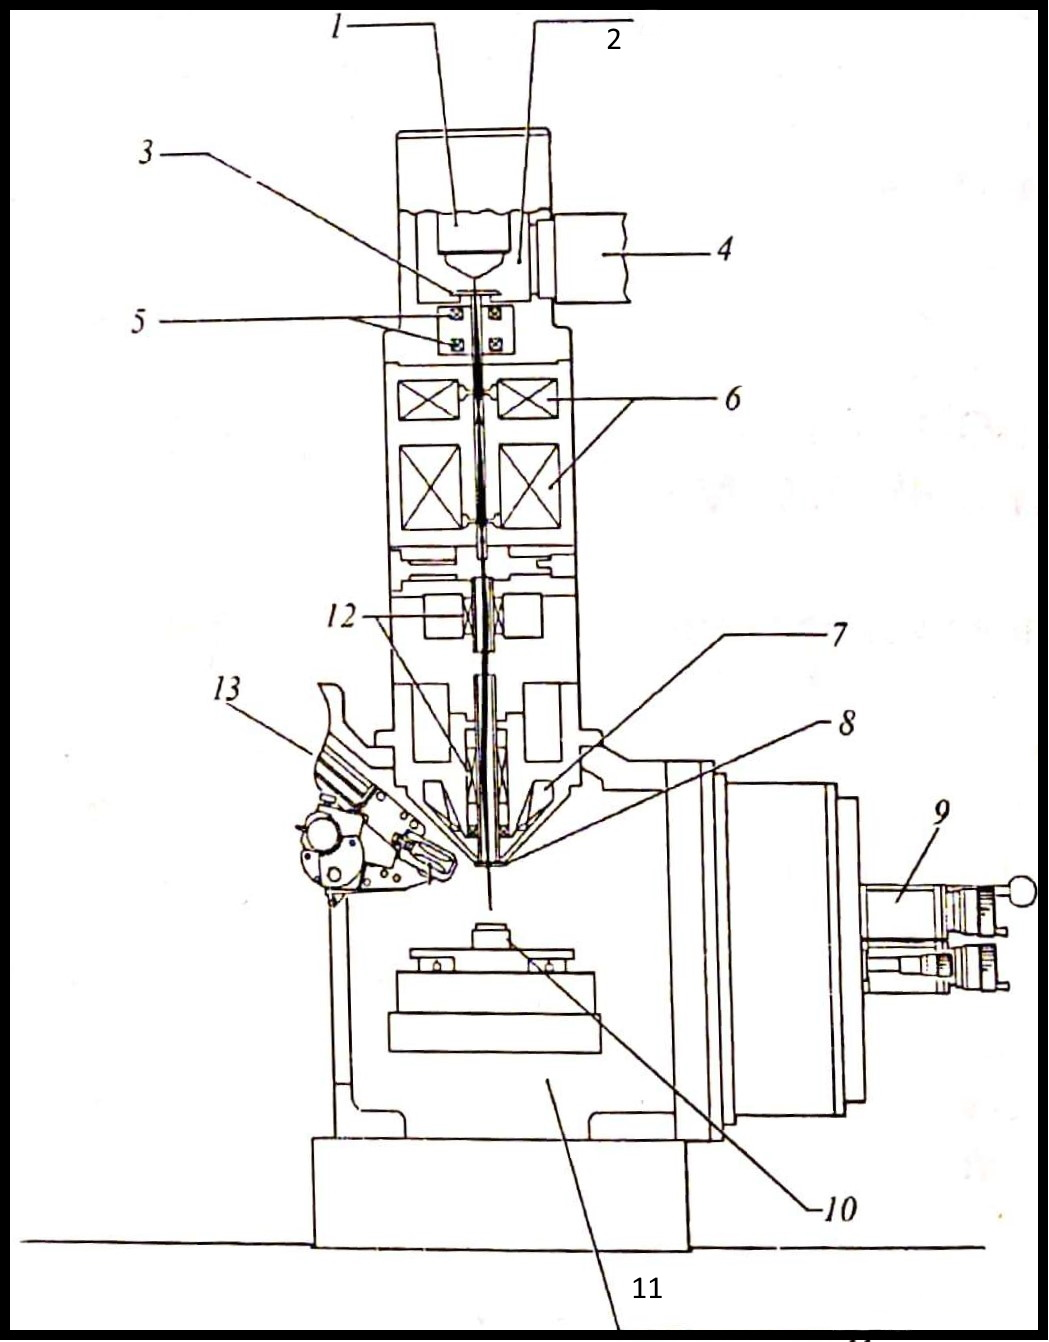
\includegraphics[scale=0.3]{pic1.jpg}
		\caption{Общая схема растрового электронного микроскопа. 1-электронная пушка; 2-камера электронной пушки; 3-анод; 4-вакуумная магистраль; 5-юстировочные катушки; 6-конденсаторные линзы; 7-объектная линза; 8-детектор упругоотраженных электронов; 9-система позиционирования образцов; 10-держатель образцов; 11-основная вакуумная камера; 12-сканирующие катушки; 13-рентгеновский спектрометр}
		\label{pic1}
	\end{figure}

\begin{figure}[h!]
	\centering
	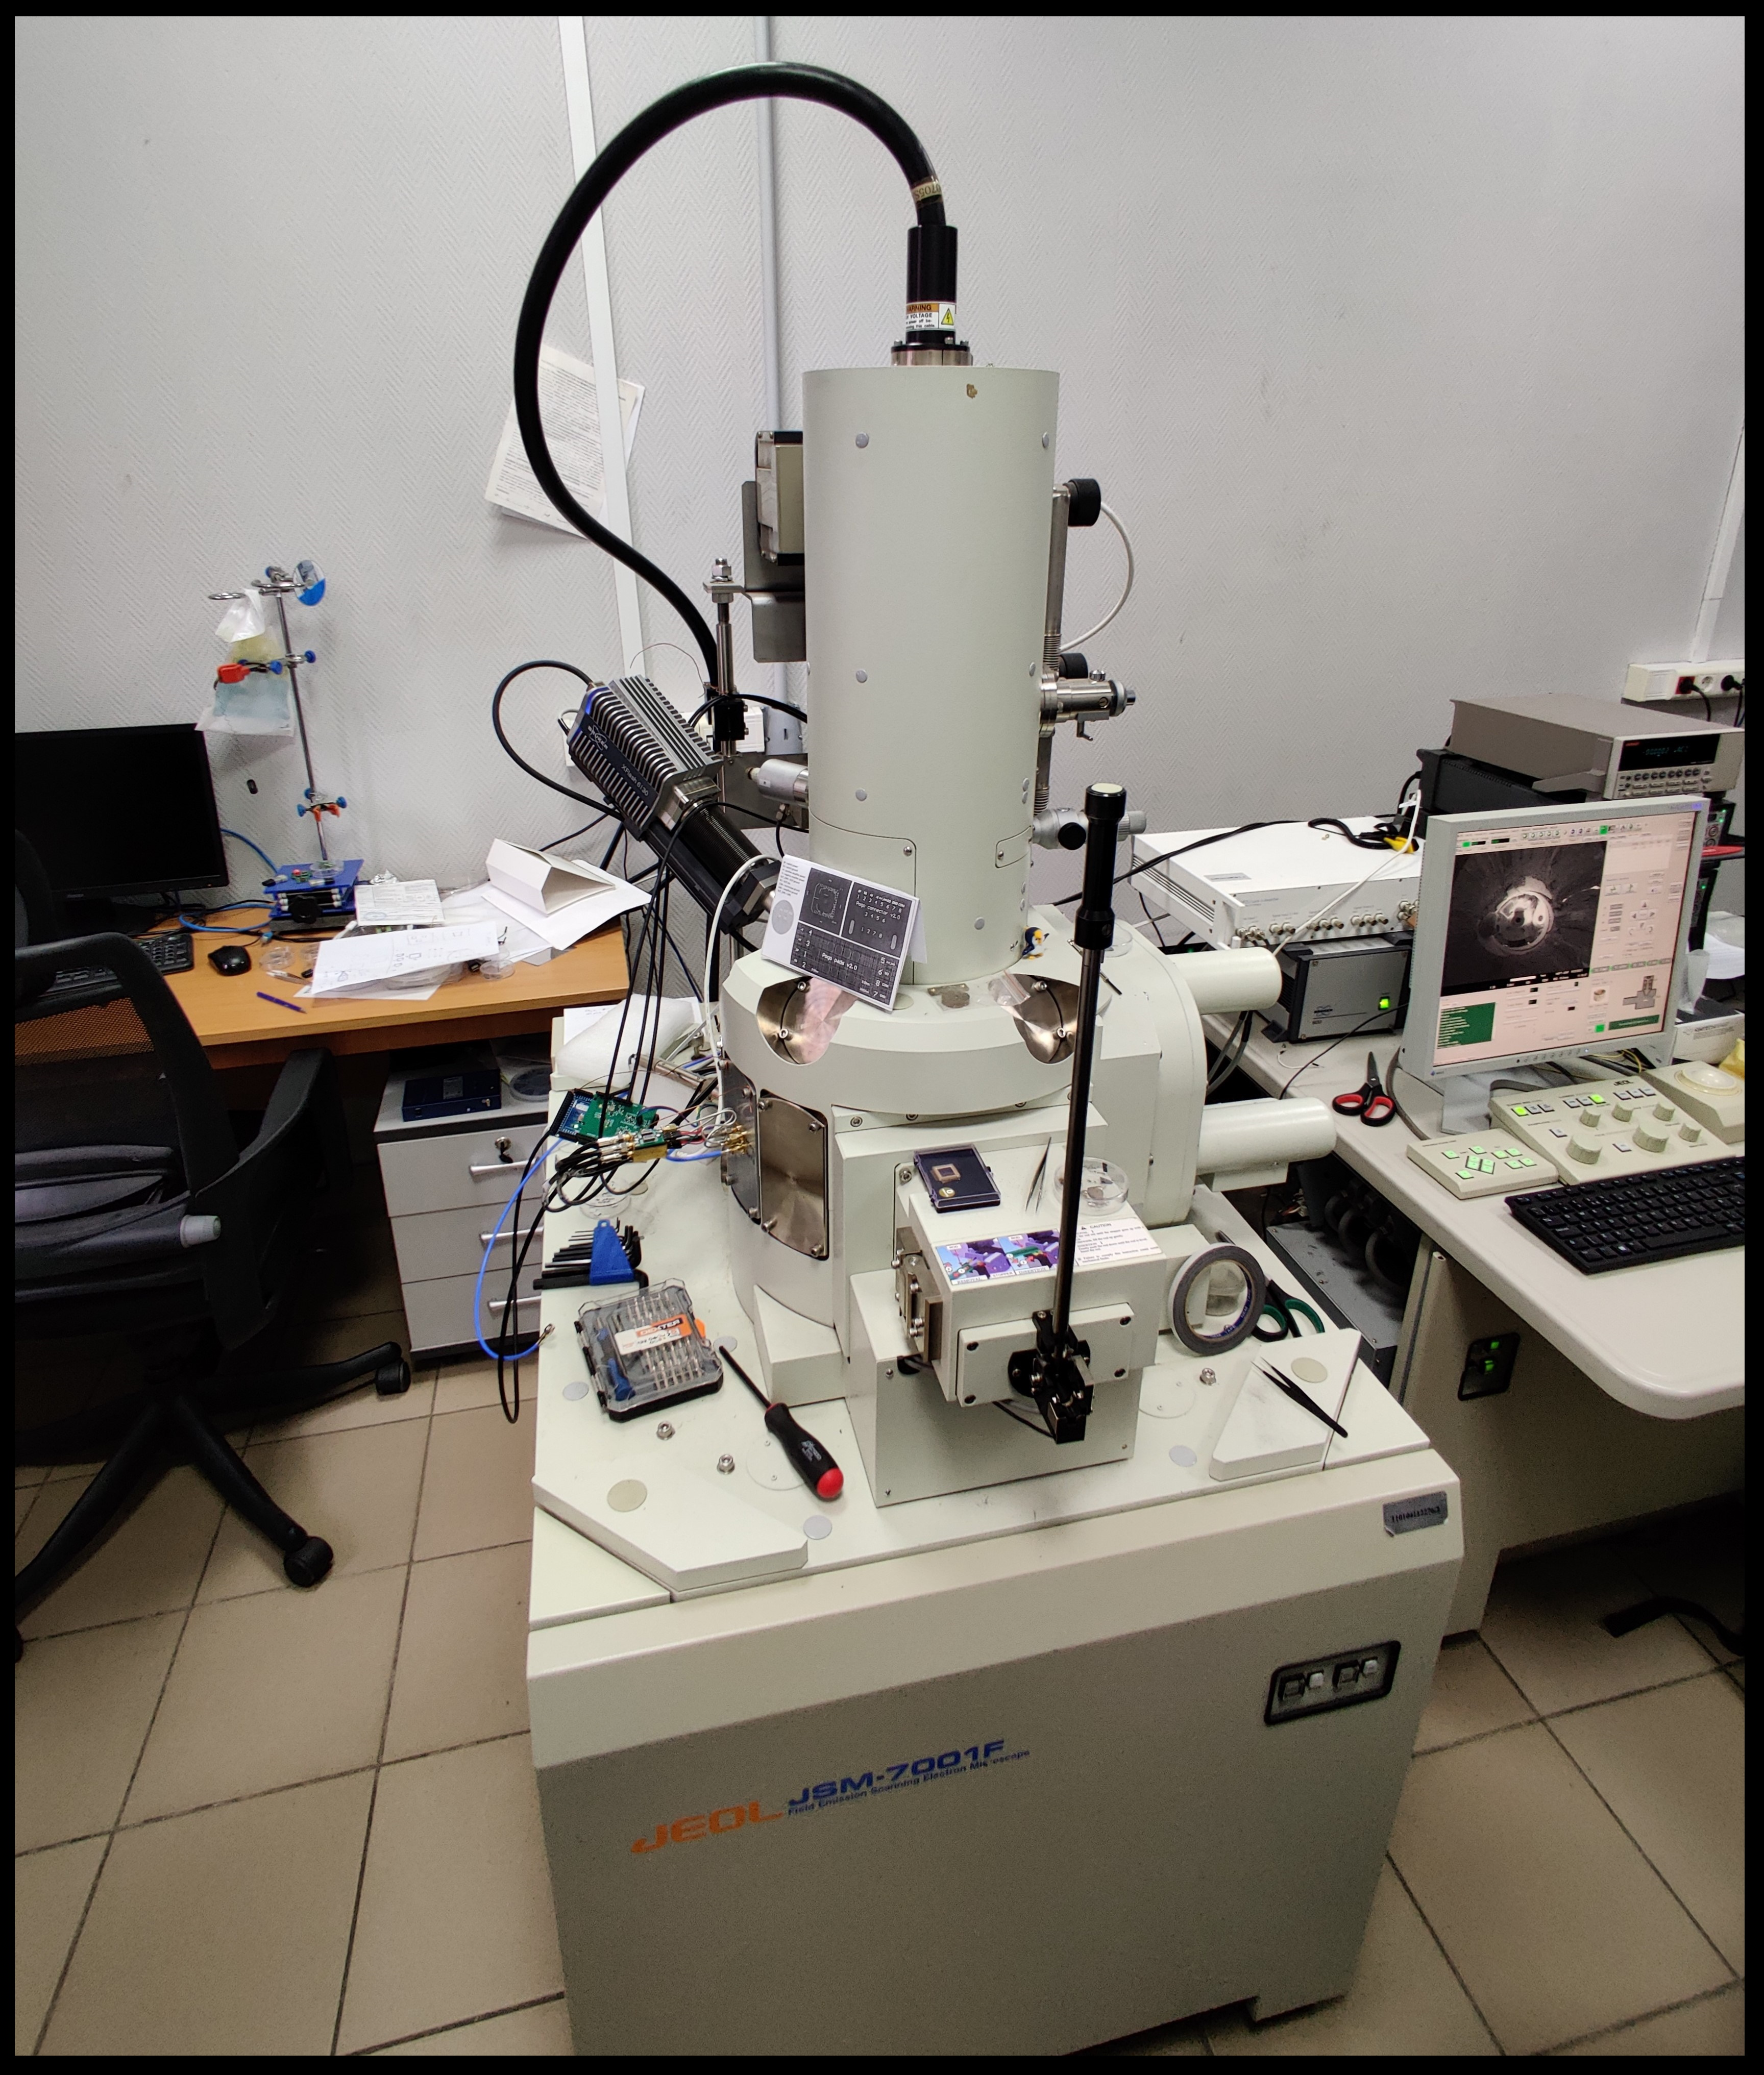
\includegraphics[scale=0.13]{pic2.jpg}
	\caption{Фотография экспериментальной установки}
	\label{pic2}
\end{figure}
Образец крепится в специальном держателе, позволящем максимально удобно оперировать с образцами в процессе работы. Образец окружен детектирующей аппаратурой-детектором отраженных электронов, детектором вторичных электронов, рентгеновским спектрометром. 
\section{Ход работы}
\subsection{Подготовка к измерениям}
Перед проведением микроскопии необходимо поместить образец в основную камеру. Для этого предназначена система позиционирования образцов 9. Давление в шлюзе поднимается до атмосферного, путем открытия электронного клапана, открывается шлюз, на подложку устанавливаются образец. В нашей работе это часть мотылька, таблетка, состоящая из двух неизвестных металлов, два монокристаллических образца кремния, пенопластовый шарик. Шлюз закрывается, начинвется откачка шлюзовой камеры с образцами. 


В установке используется один форвакуумный насос, поэтому, чтобы не испортить вакуум в основной вакуумной камере, она отделяется заслонкой от насоса и начинается откачка. Когда давления в шлюзе и основной камере сравняются- система откроет соединяющий клапан и давления выравняются. 

После достижения рабочего давления ($ \approx 1\e{-4}\s Па $) и открытия клапана, соединяющего шлюз с основной камерой, образцы перемещаются в рабочую зону с помощью рычага. 

В программном обеспечении устанавливается параметр offset=4 мм, отвечающий за высоту таблетки с образцами. Можно приступать к микроскопии. 
\subsection{Микроскопия}
\subsubsection{Крыло мотылька}
\begin{figure}[h!]
	\centering
	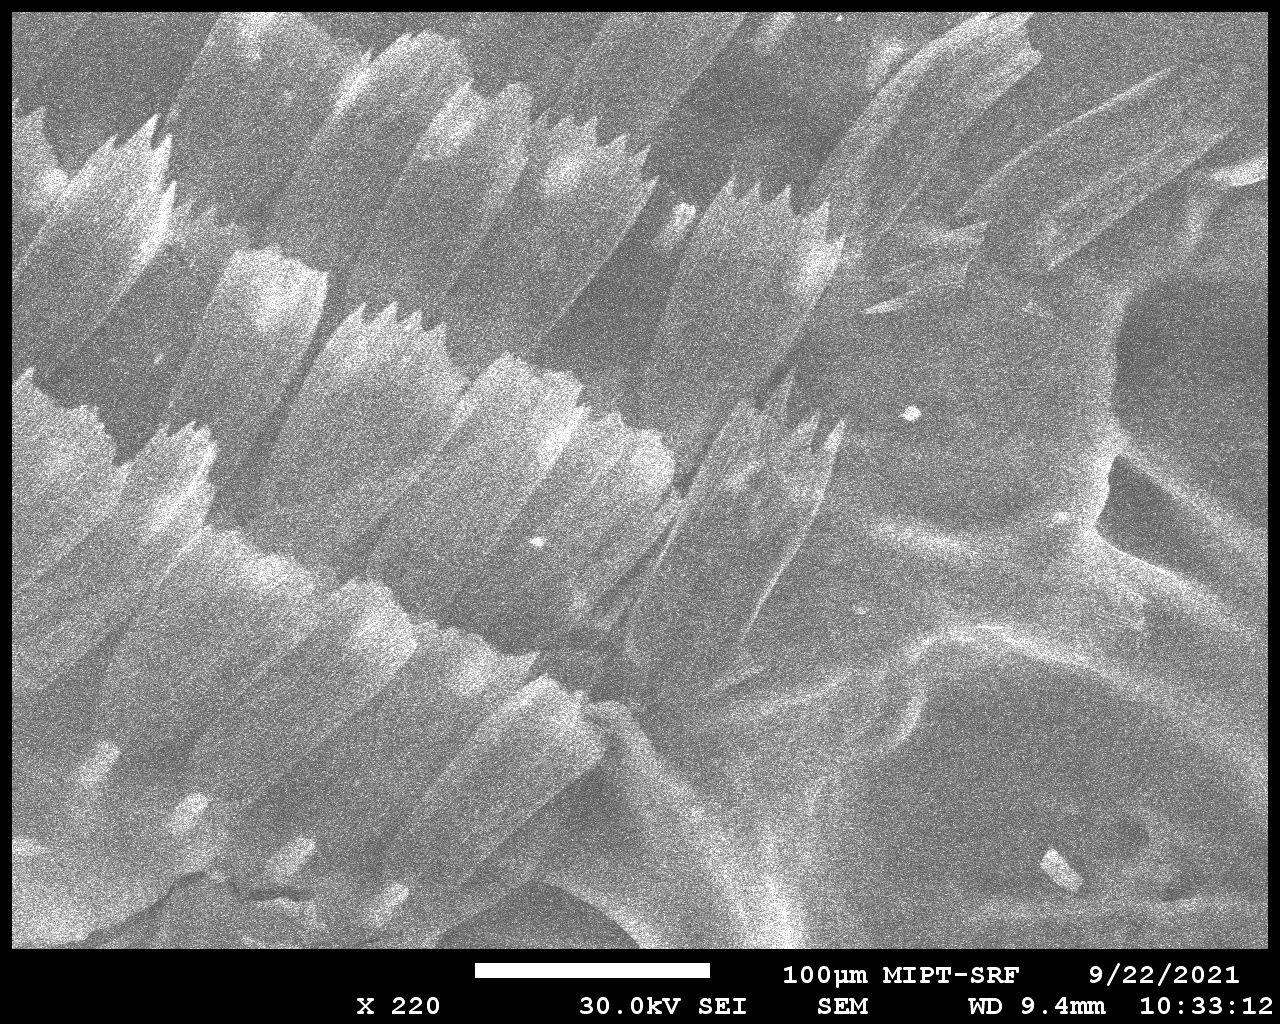
\includegraphics[scale=1.3]{pic3.jpg}
	\caption{Крыло мотылька. Быстрый режим сканирования}
	\label{pic3}
\end{figure}
На \picref{pic3} изображен результат сканирования крыла мотылька в режиме истинно вторичных электронов (SEI). Изображение зашумлено, однако отчетливо видны отдельные чешуйки ($ \approx 100\s мкм $) из которых состоит крыло.
\begin{figure}[h!]
	\centering
	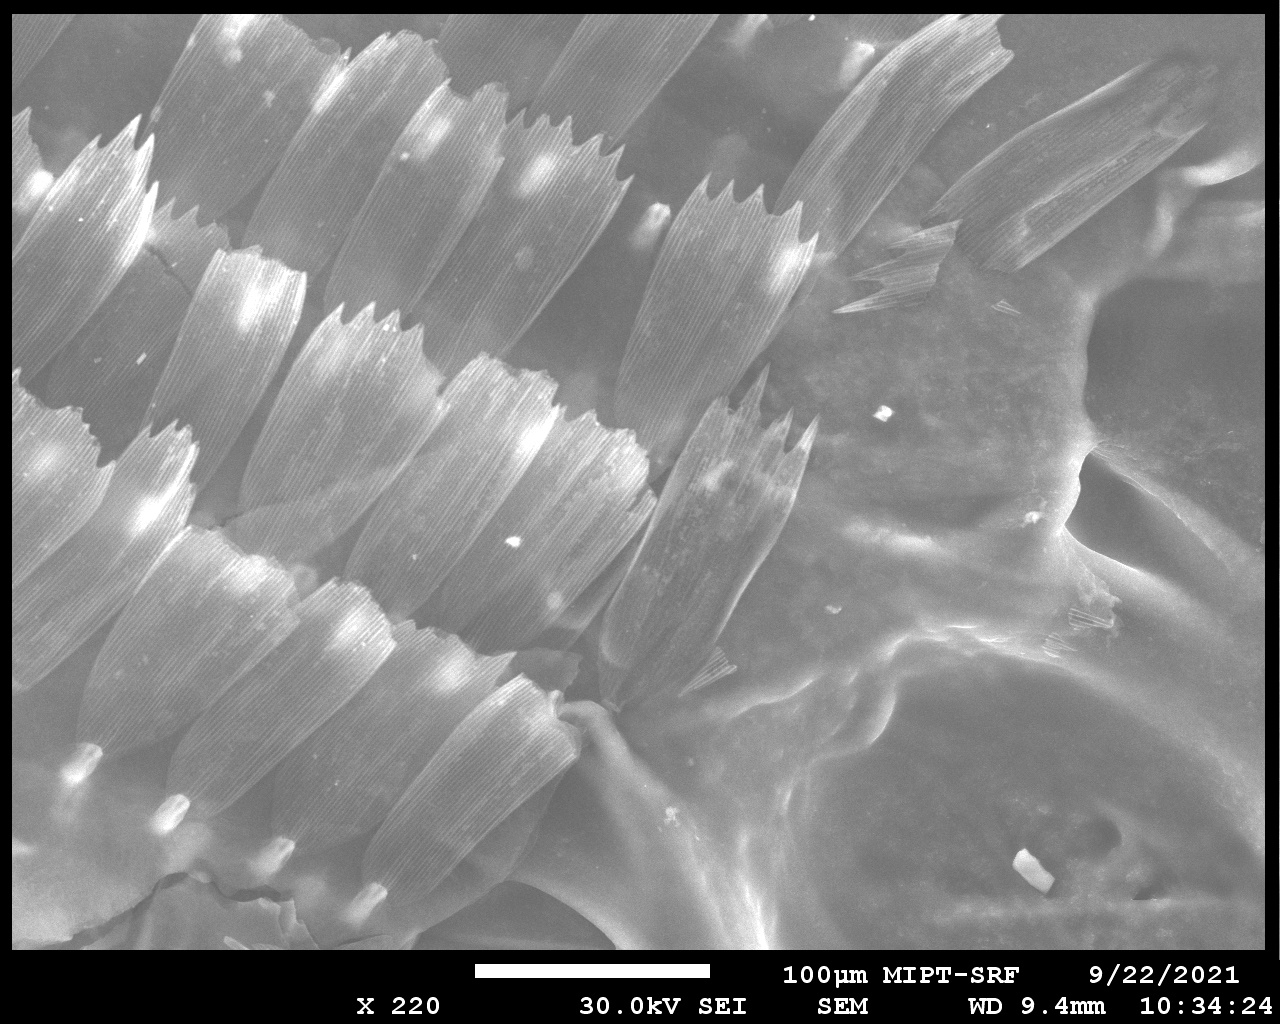
\includegraphics[scale=1.3]{pic4.jpg}
	\caption{Круло мотылька. Медленный режим сканирования}
	\label{pic4}
\end{figure}
Для получения более детального изображения, переключимся в режим медленного сканирования \picref{pic4}. Изображение стало менее шумным и теперь стало возможным расмотреть структуру отдельной чешуйки - она состоит из продольных канальцев.

При приближенном рассмотрении одного из таких канальцев \picref{pic5} становится видна пористая структура, заполняющая пространство между направляющими канальцами. Характерный размер пор $ \approx 500\s нм $, что соизмеримо с длиной волны видимого излучения. Это объясняет переливающийся окрас крыльев бабочки - на этих порах происходит дифракция видимого диапазона излучения.
\begin{figure}[h!]
	\centering
	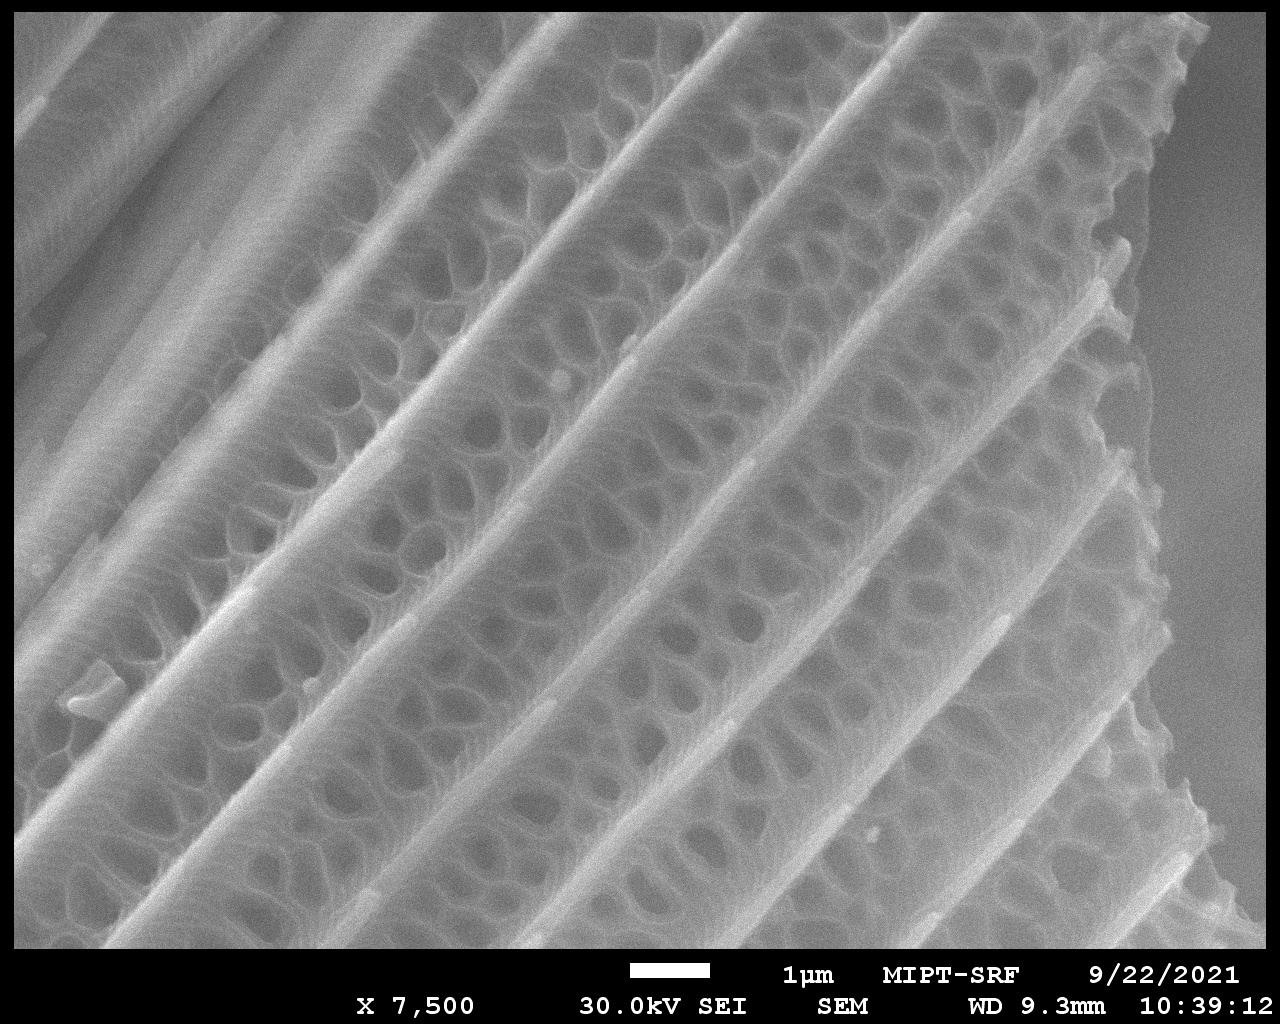
\includegraphics[scale=1.3]{pic5.jpg}
	\caption{Крыло мотылька. Структура отдельной чешуйки}
	\label{pic5}
\end{figure}
\subsubsection{Таблетка из двух металлов}

\begin{figure}[h!]
	\centering
	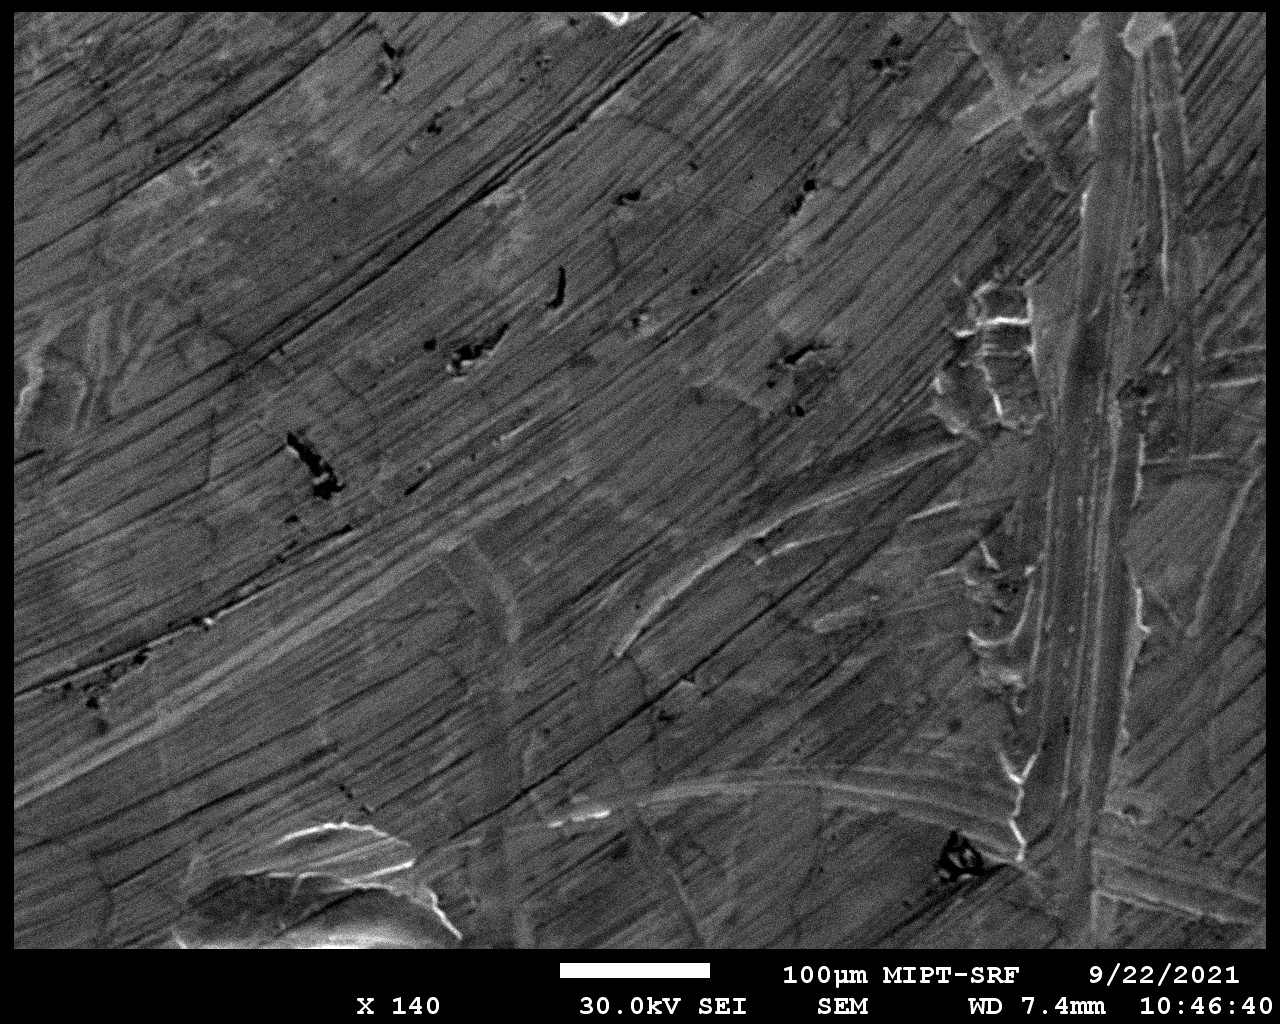
\includegraphics[scale=1.3]{pic6.jpg}
	\caption{Таблетка из двух металлов}
	\label{pic6}
\end{figure}
На \picref{pic6} изображен контрольный скан таблетки в режиме вторичных электронов. На скане присутствует информация как о рельефе, так и о элементном составе образца, но в перемешанной и трудноинтерпретируемой форме. Для получения раздельной информации о рельефе и о составе образца, переключимся в режим сбора упругоотраженных электронов (BSE). Для этого в основную камеру необходимо ввести датчик упругоотраженных электронов, имеющий форму двухсекционного диска. 

\begin{figure}[h!]
	\centering
	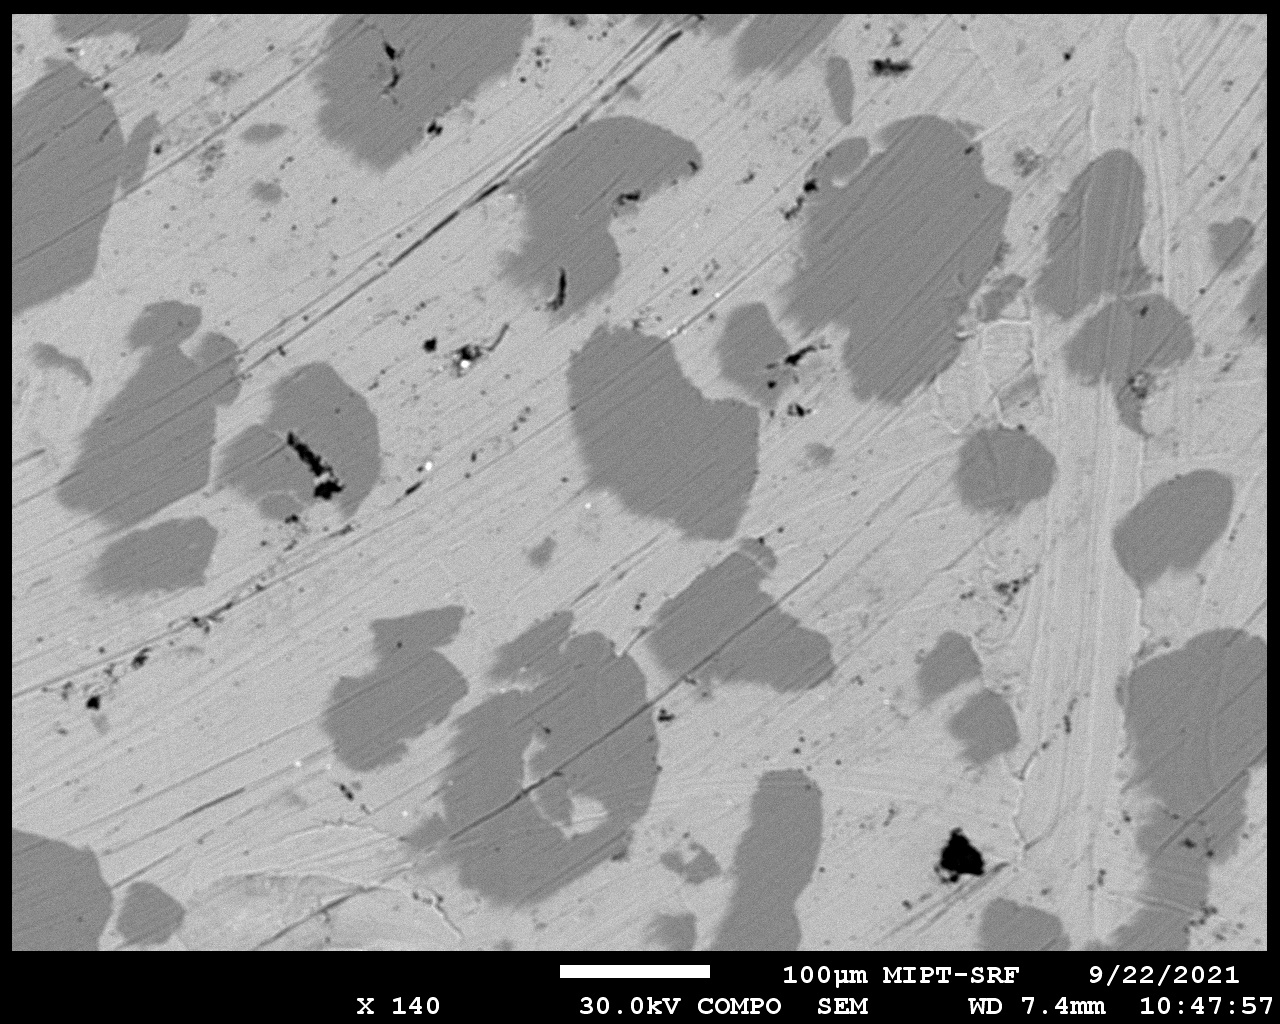
\includegraphics[scale=1]{pic7.jpg}
	\caption{Таблетка. Z-контраст}
	\label{pic7}
\end{figure}
\begin{figure}[h!]
	\centering
	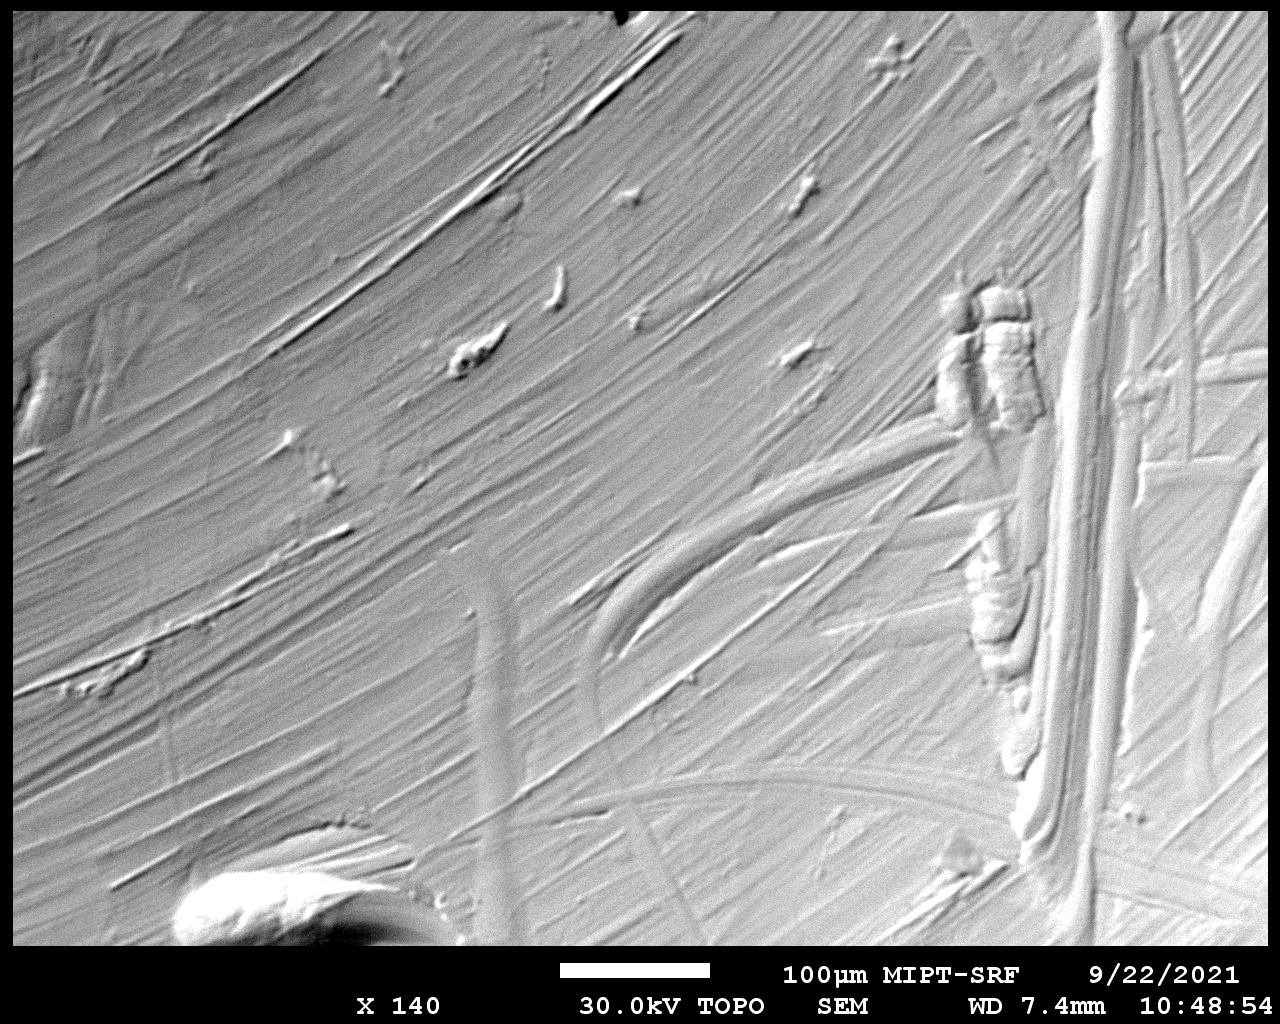
\includegraphics[scale=1]{pic8.jpg}
	\caption{Таблетка. Топологический контраст}
	\label{pic8}
\end{figure}

В режиме Z-контраста \picref{pic7}  отчетливо видны темные пятна- участки с другим химическим составом. Особенности рельефа также заметны, но в меньшей степени. В режиме топологического контраста \picref{pic8} отчетливо видны все особенности рельефа, а информация о различном составе полностью отсутствует.

Для определения элементного состава образца, воспользуемся рентгеноспектрыльным анализом. 

\begin{figure}[h!]
	\centering
	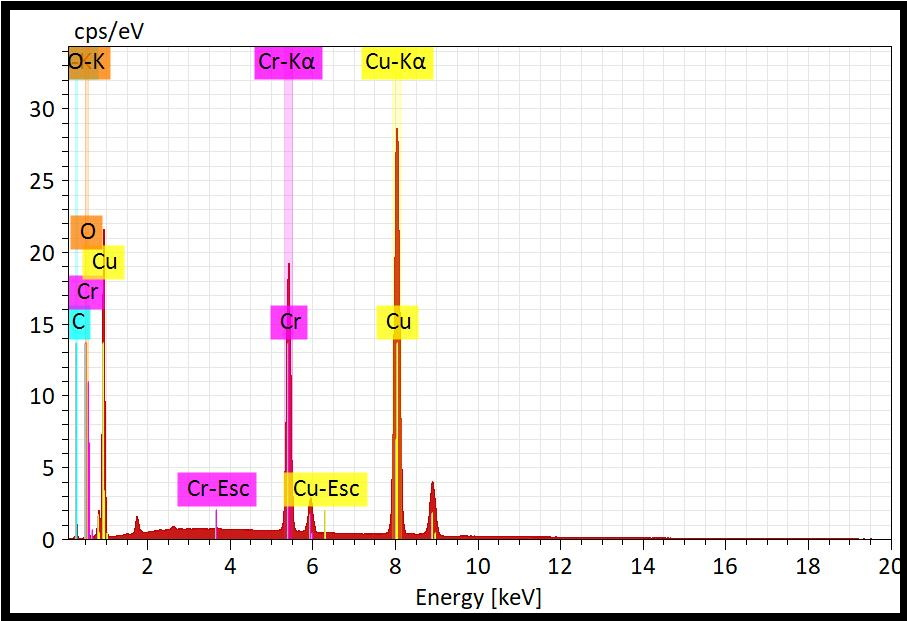
\includegraphics[scale=0.6]{pic9.jpg}
	\caption{Спектр ренгеновского излучения}
	\label{pic9}
\end{figure} 
\begin{figure}[h!]
	\centering
	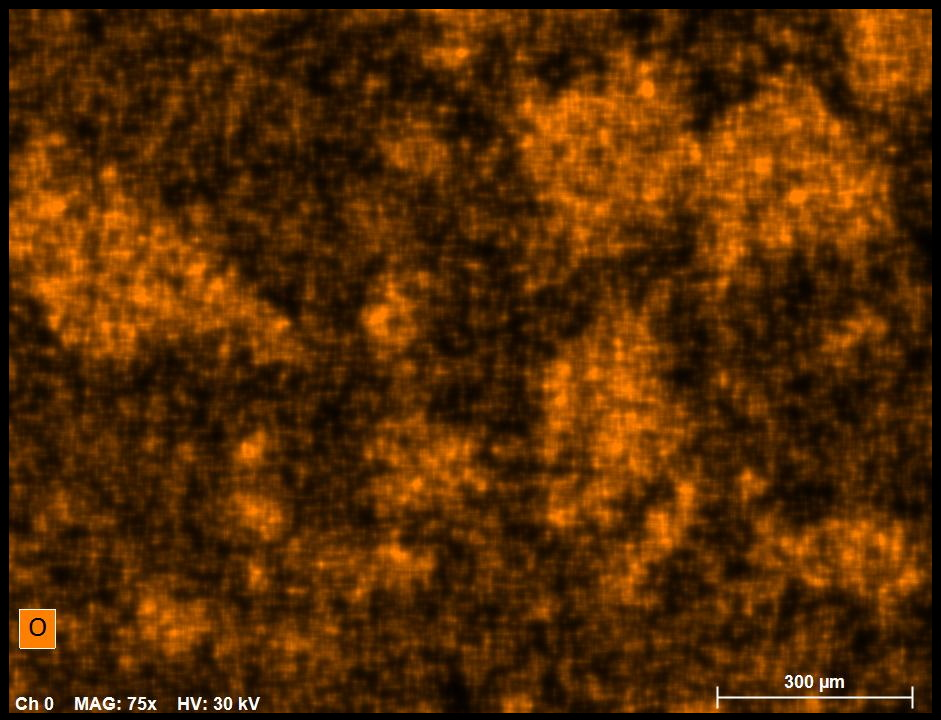
\includegraphics[scale=0.6]{pic10.jpg}
	\caption{Таблетка. Карта кислорода}
	\label{pic10}
\end{figure}
\begin{figure}[h!]
	\centering
	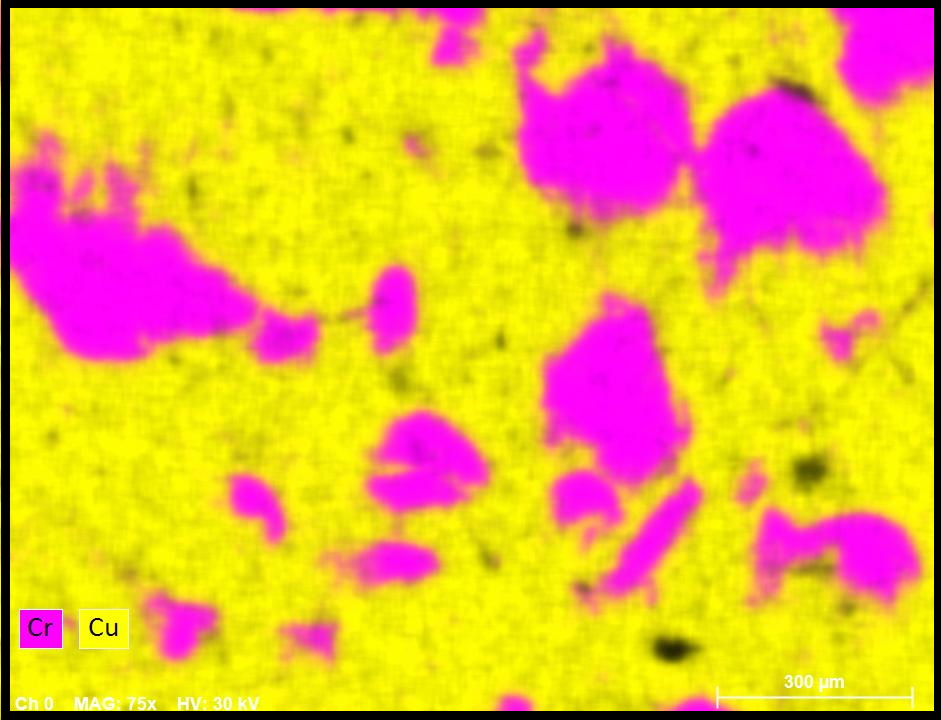
\includegraphics[scale=0.6]{pic11.jpg}
	\caption{Таблетка. Карта хрома и меди}
	\label{pic11}
\end{figure}


На спектрограмме отчеливо видны пики кислорода, углерода,хрома и меди. Кислород и углерод попали на образец из внешней среды. Хром и медь - материалы из которых изготовлена таблетка. Чтобы в этом убедиться, рассмотрим карту меди и хрома \picref{pic10}. Образец состоит из меди с вкраплениями хрома. 

Заметим также один любоптыный эффект. На карте кислорода \picref{pic9} области повышенной концентрации кислорода соответствуют вкраплениям хрома. Это можно объснить повышенной адсорбционной способностью хрома по сравнению с кислородом или разной скоростью/толщиной образования оксидной пленки на поверхности металлов. 

\subsubsection{Монокристаллы кремния}
Для исследования образцов кремния, зафиксируем электронный луч в одной точке, заставив его освещать образец под разными углами. На \picref{pic12} и \picref{pic13} видны симметричные полосы, причем на первом образце их 4, а на втором 3. Эти полосы - направления вдоль граней монокристалла, появившиеся в результате эффекта каналирования первичных электронов.

На \picref{pic12} более узкие полосы соответствуют основным направлениям граням куба, а более широкие- диагональные направления.

На \picref{pic13} наблюдается симметрия 6-го порядка. Это объясняется тем, что кристалл выращен таким образом, что его вершина (<<кубика>>) направлена вверх 

\begin{figure}[h!]
	\centering
	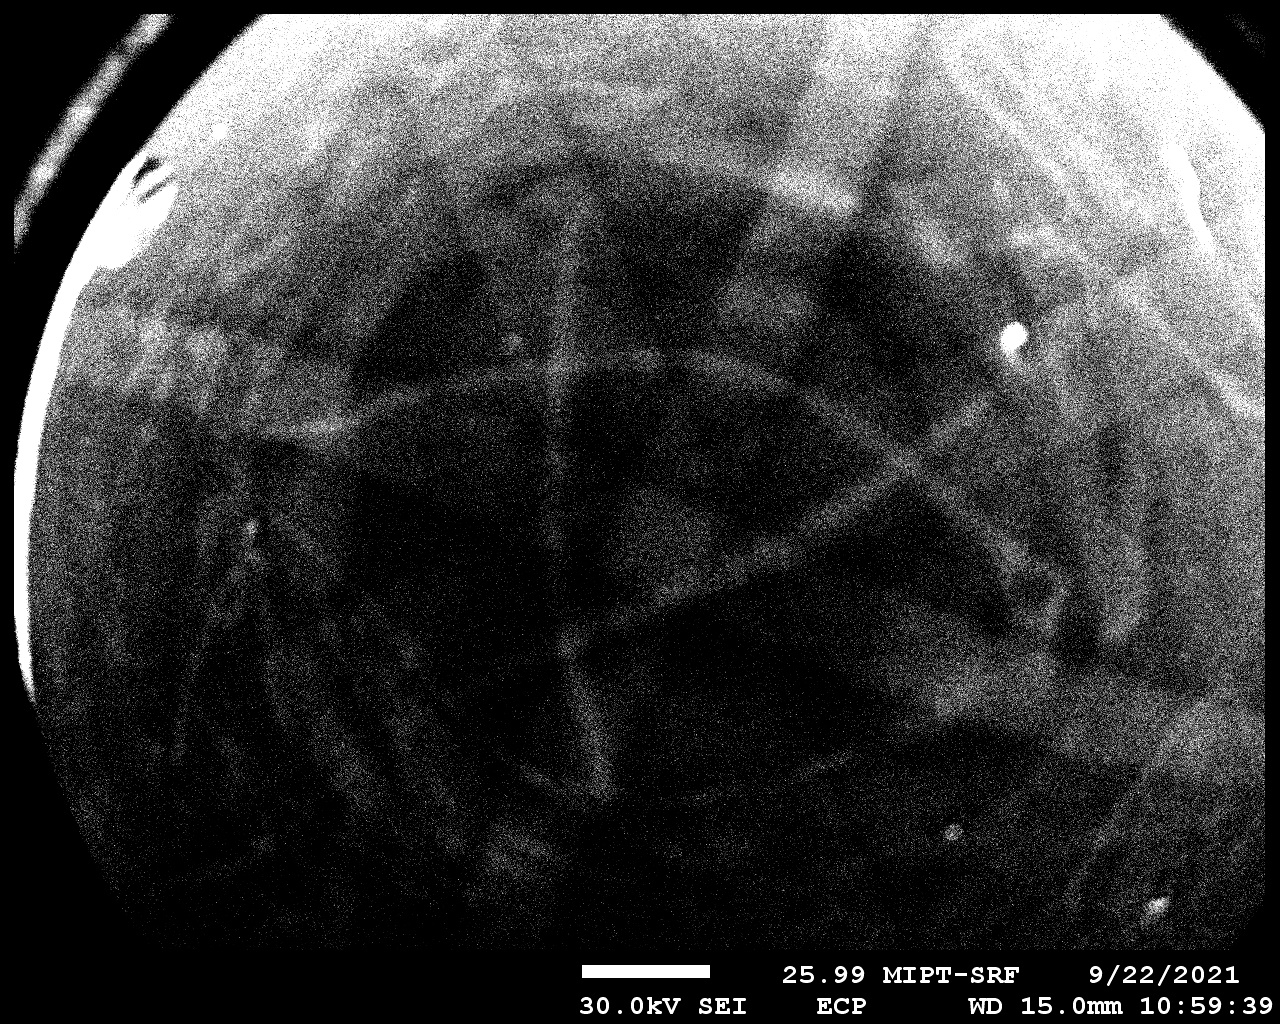
\includegraphics[scale=1]{pic12.jpg}
	\caption{Монокристан кремния гранью вверх}
	\label{pic12}
\end{figure}
\begin{figure}[h!]
	\centering
	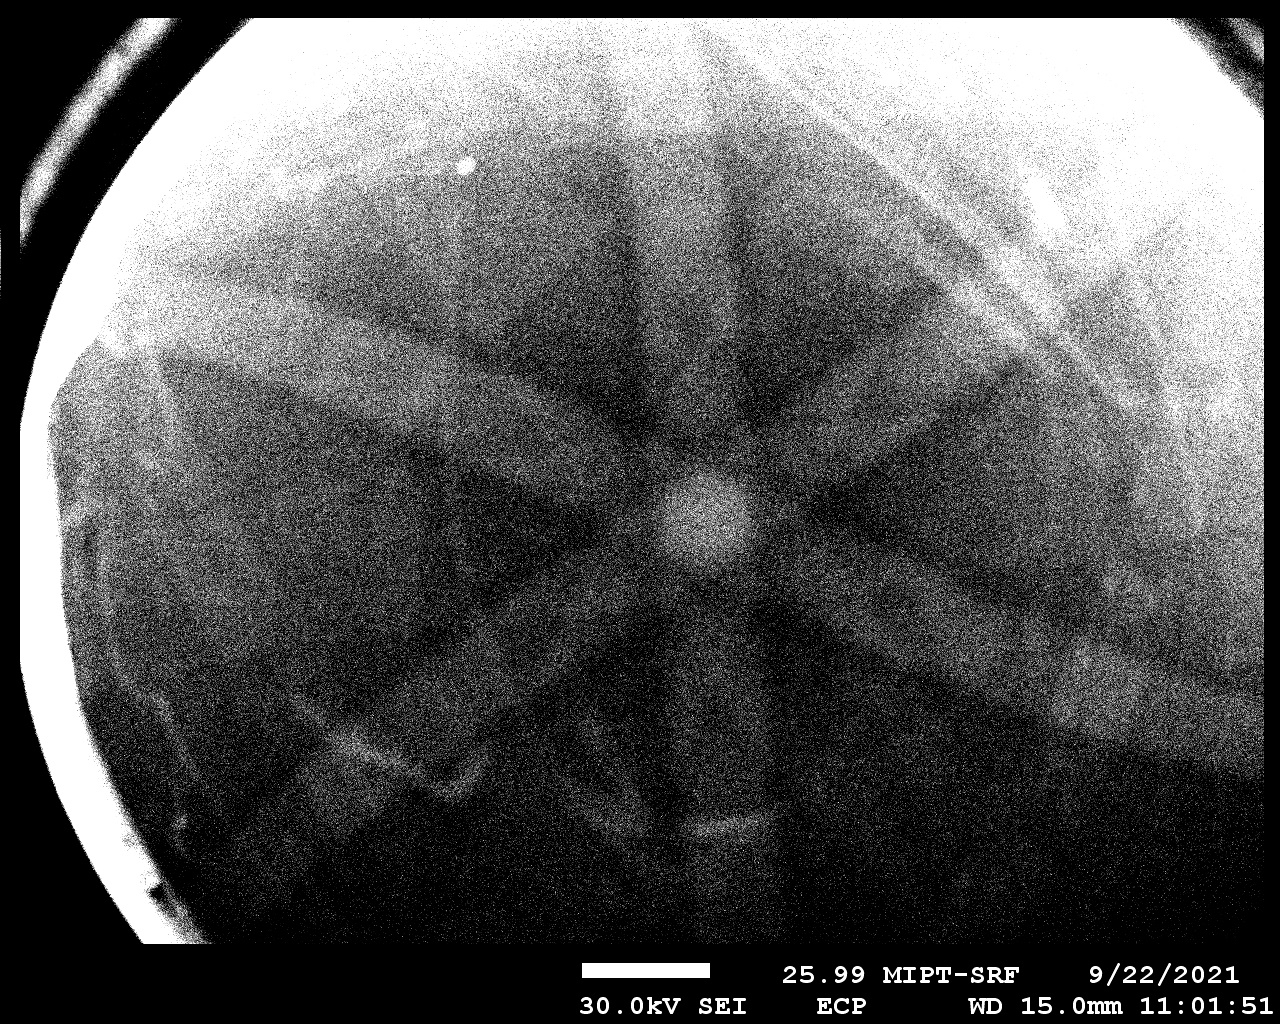
\includegraphics[scale=1]{pic13.jpg}
	\caption{Монокристал кремния вершиной вверх}
	\label{pic13}
\end{figure}

\subsubsection{Пенопласт}
Отличительным свойством этого образца \picref{pic14} является то, что это диэлектрик. Вследствии этого, в процессе сканирования, на образце накапливается отрицатльный заряд, который своим полем начинает искажать траекторию движения первичных электронов, что ведет к деформации изображения, а именно к его сжатию.


\begin{figure}[h!]
	\centering
	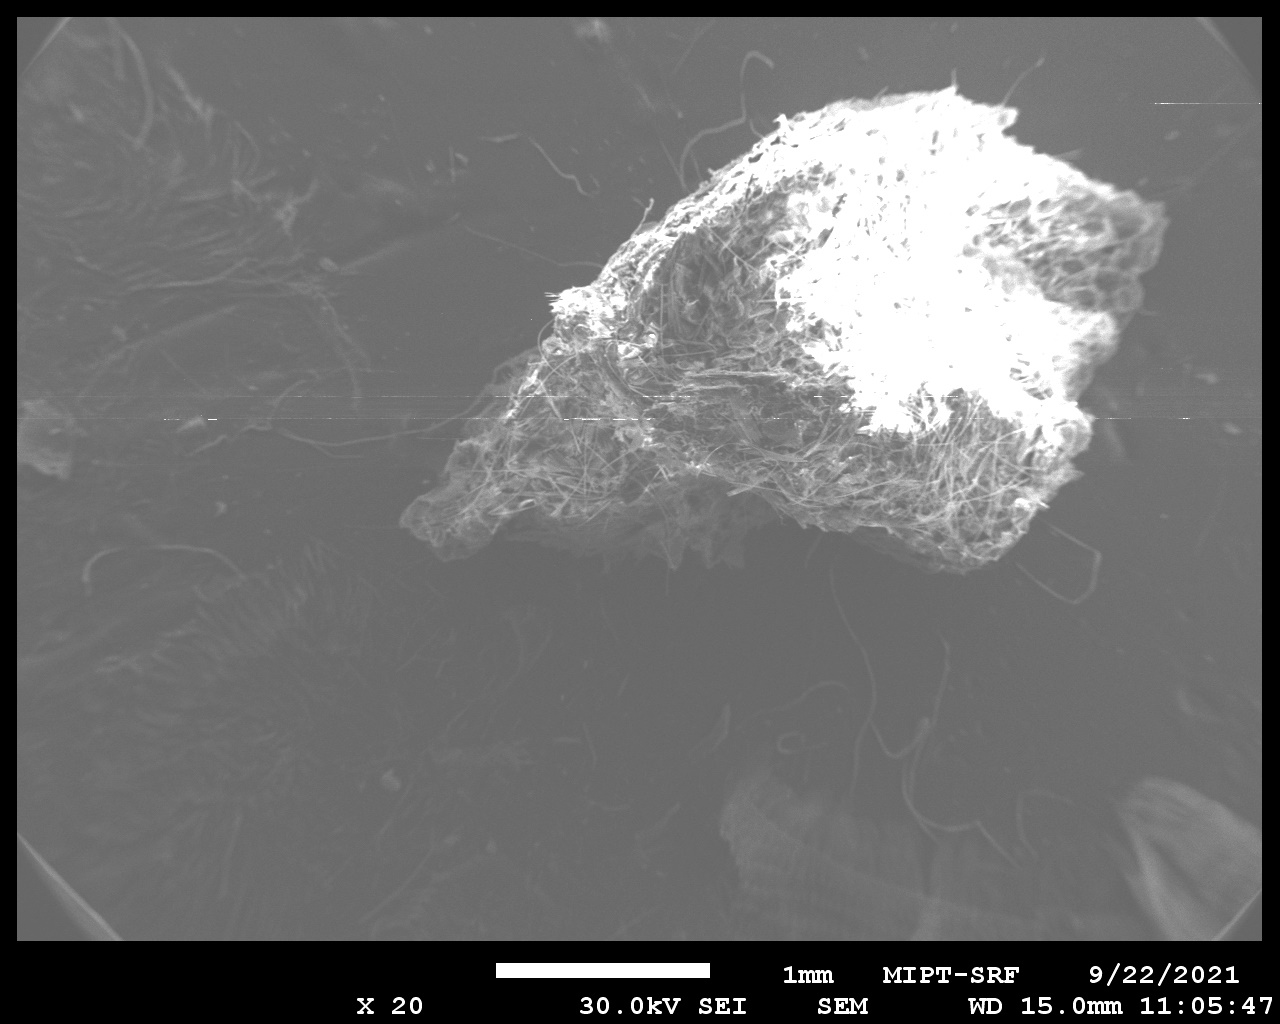
\includegraphics[scale=1]{pic14.jpg}
	\caption{Пенопласт}
	\label{pic14}
\end{figure}

Можно пронаблюдать интересный эффект, если начать постепенно понижать энергию первичных электронов. Изображение вначаче деформируется до неузнаваемости, а затем в нем начнет проявляться изображение верхней внутренней части микроскопа- отверстие колонны, детектор вторичных электронов, детектор упругоотраженных электронов и рентгеновский детектор.
\begin{figure}[h!]
	\centering
	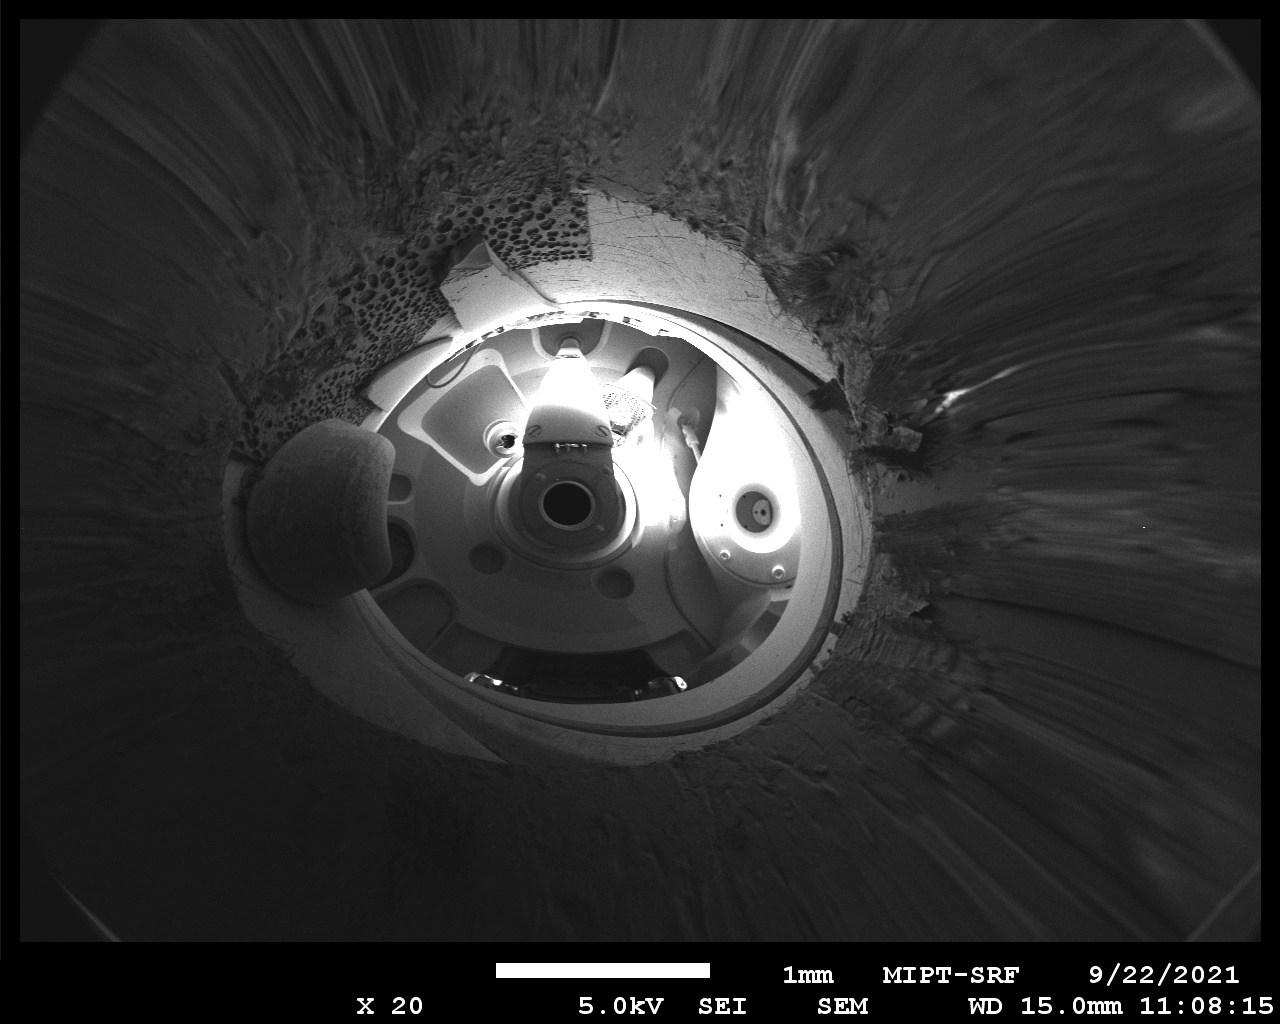
\includegraphics[scale=1]{pic15.jpg}
	\caption{Эффект <<Зеркала>>}
	\label{pic15}
\end{figure}

\begin{figure}[h!]
	\centering
	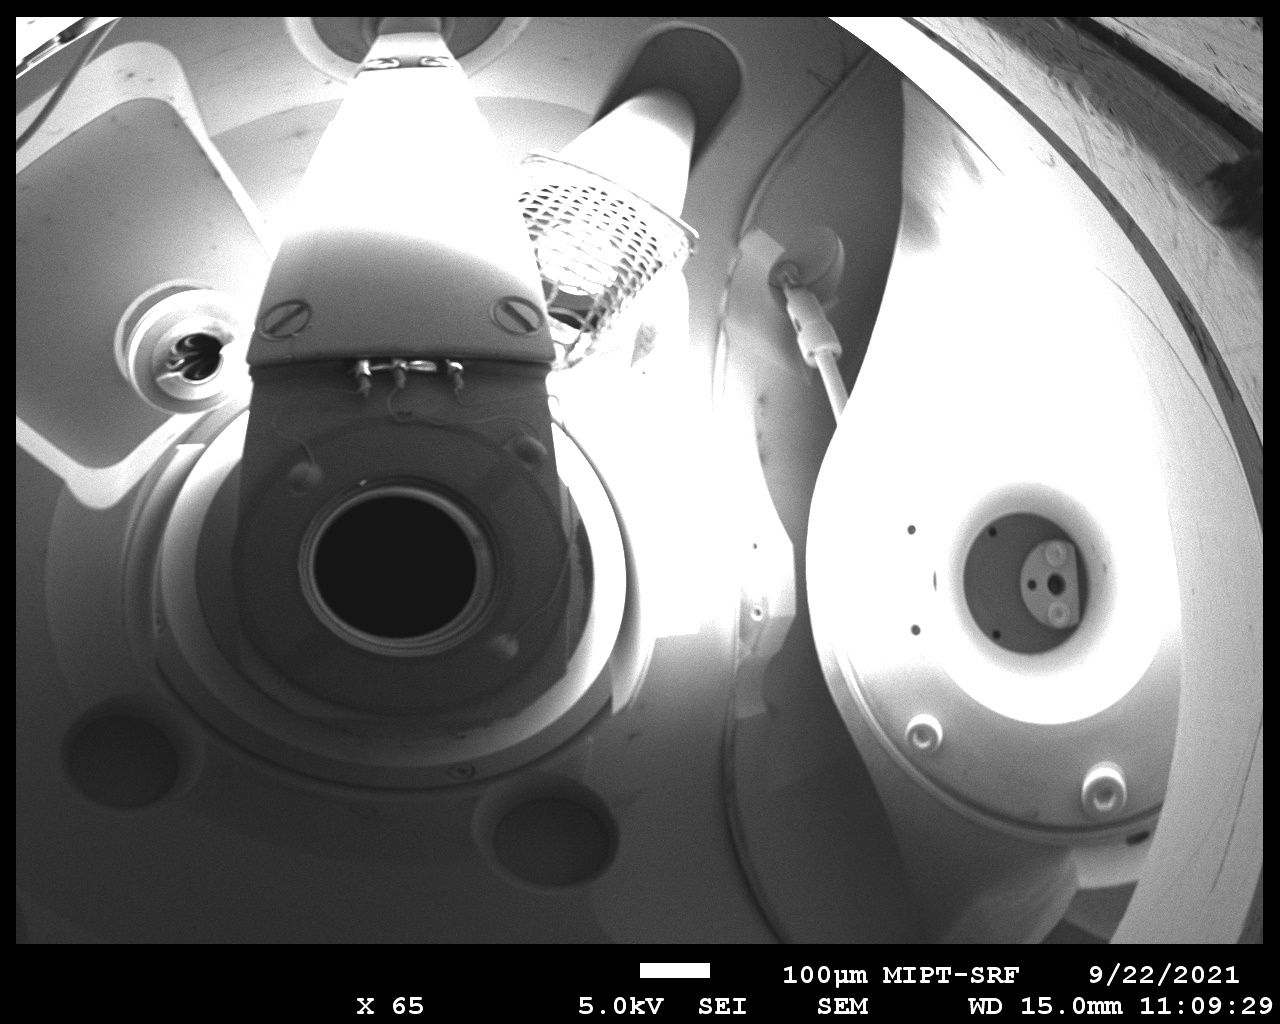
\includegraphics[scale=1]{pic16.jpg}
	\caption{Эффект <<Зеркала>>}
	\label{pic16}
\end{figure}


Эффект объясняется тем, что при большой величине накопленного отрицательного заряда электроны первичного пучка не попадают на образец. Т.е. участок образца играет роль зеркала для электронов, что привоит к формированию изображения окружающих деталей камеры микроскопа.






	
	
\end{document}